The purpose of this lecture is to introduce some tools for solving 3D geometry problems. Although adding a dimension to 2D seems like it would complicate a lot of things, we actually use much of the same tools we use in 2D, albeit with some different considerations. This lecture is more of a mix of 3D geometry rather than a fixed focus, but that's because I want to introduce you to a lot of topics. This lecture is also more problem-solving based, because the foundation for 3D geometry is actually really simple. It's the application that takes a lot of work getting good at.

\subsection{Coordinate Systems}

In the \textbf{Cartesian Plane}, we are accustomed to denoting a point by a pair of coordinates, usually $(x,y)$.

\begin{figure}[H]
  \centering
  \begin{minipage}[b]{0.4\textwidth}
    \centering
    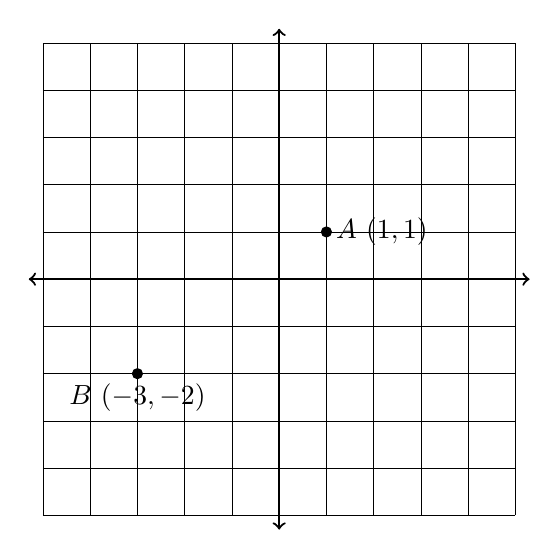
\begin{tikzpicture}[scale=0.6]
    \draw[very thin] (-5,-5) grid (5,5);
    \draw[fill] (1,1) circle [radius=3pt];
    \node[above,right] at (1,1) {$A$ $(1, 1)$};
    \draw[fill] (-3,-2) circle [radius=3pt];
    \node[below] at (-3,-2) {$B$ $(-3, -2)$};
    \draw[<->,thick] (0,-5.3)--(0,5.3);
    \draw[<->,thick] (-5.3,0)--(5.3 ,0);
    \end{tikzpicture}
    \caption{Two points on a Cartesian Plane}
  \end{minipage}
  \hfill
  \begin{minipage}[b]{0.4\textwidth}
    \centering
    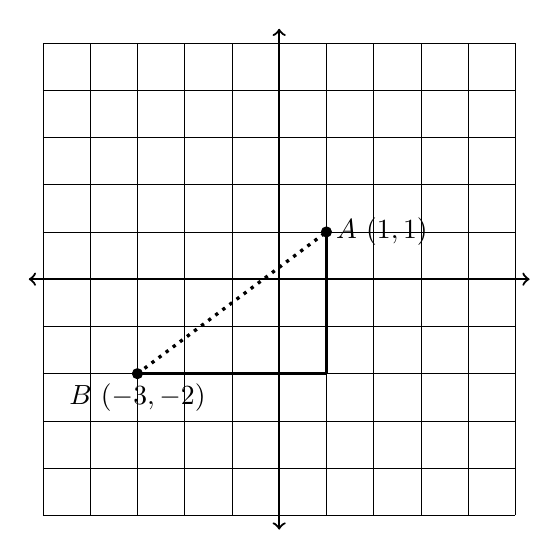
\begin{tikzpicture}[scale=0.6]
    \draw[very thin] (-5,-5) grid (5,5);
    \draw[fill] (1,1) circle [radius=3pt];
    \node[above,right] at (1,1) {$A$ $(1, 1)$};
    \draw[fill] (-3,-2) circle [radius=3pt];
    \node[below] at (-3,-2) {$B$ $(-3, -2)$};
    \draw[<->,thick] (0,-5.3)--(0,5.3);
    \draw[<->,thick] (-5.3,0)--(5.3 ,0);
    \draw[very thick] (-3,-2)--(1,-2);
    \draw[very thick] (1,-2)--(1,1);
    \draw[dotted, very thick] (-3,-2)--(1,1);
    \end{tikzpicture}
    \caption{Use of the Pythagorean Theorem}
    \label{fig:pyth}
  \end{minipage}
\end{figure}

\subsubsection{Distance}

When we want to find the distance between two points, we can employ Pythagorean Theorem as shown in Figure \ref{fig:pyth}. From the right triangle, it is clear that the distance between any points is

$$\abs{\overline{AB}}=\sqrt{\abs{B_x-A_x}^2+\abs{B_y-A_y}^2}$$

Or more commonly written as, given two points $P_1=(x_1,y_1),P_2=(x_2,y_2)$,

\begin{equation}
    \boxed{D(P_1,P_2)=\sqrt{(x_2-x_1)^2+(y_2-y_1)^2}}.
\end{equation}

Note that because of the square of the difference, the order of $x_2-x_1$ does not really matter. I like to think of it as just the absolute value of the two $x$ coordinates squared (because it has to be positive at the end).

\subsubsection{Equation of a Line}

It is important to also introduce the equation of a line in the Cartesian system. There are three forms of the line equation that you have to know. 

\begin{enumerate}
    \item \textbf{Slope Intercept:} $y = mx+b$, where $m=\frac{y_2-y_1}{x_2-x_1}$ is the slope and $b$ is the $y$-intercept (when the line intersects the $y$ axis). This is the most convenient form to have since it tells you so much information.
    \item \textbf{Point-Slope:} $(y-y_1)=m(x-x_1)$, where $m$ is the slope. This form is convenient when you are given two points, because you can easily find the slope and then all you have to do is plug in a point into the equation.
    \item \textbf{Standard Form:} $Ax+By=C$. This is the ``pretty'' form, but doesn't really give us much information, except that you can find the $x$ and $y$-intercepts really easily by setting either one to zero.
\end{enumerate}
%enumerate: Slope intercept, point slope, standard + their advantages

\subsubsection{Coordinate Bashing}
Sometimes when you have no idea what to do for a geometry problem, you can always employ a \textbf{coordinate bash}. Usually, the process goes something like this:
\begin{enumerate}
    \item Write down equations for lines
    \item Find intersections of lines to find desired points
    \item Use distance formula to find distance between points and lengths of line segments
    \item If the problem asks for areas, employ Heron's, determinants, or shoelace 
\end{enumerate}

Note that when you use coordinate bash, you are almost \textit{certainly not using the best method to solve the problem}. Which means that only when you are \textit{desperate} and have time should you consider this method.

\begin{problem}
In $\triangle ABC$, $AB=13,AC=15,BC=14$. Let $E$ be a point on $\overline{AC}$ such that $AE:EC=1:4$, and let $M$ be the midpoint of $\overline{BC}$. Find the length of $\overline{ME}$.
\end{problem}

\subsubsection{Three Dimensions}
First, let's consider the question: what does it mean to be in a higher dimension? Well, to start off, we can easily interpret our lives as a \textbf{3D World}. We have three degrees of freedom of motion that allow us to move and feel 3D textures and all that good stuff. It turns out, we can also think of our world as 4D, because we are also moving through time, another dimension (see how abstract this is getting already?). What all this dimension business means is that each dimension gives us a direction or a \textit{degree of freedom}, something variable that can be changed. 

For our problem-solving purposes, the only definition we are really worried about is \textbf{distance} and how things are positioned relative to each other. It turns out that the Pythagorean Theorem (albeit in a different form) still works for distance in a $n$-dimensional space (you can test this out yourself by applying it twice in 3D). In general, the distance between two points $U$ and $V$ is 

\begin{equation}
    \abs{\overline{UV}} = \sqrt{\sum\limits_{i=1}^{n} (v_i-u_i)^2}
\end{equation}

Since 3D is the most common higher-dimensional geometry you'll see in competition math, the distance equation (for convenience) is

\begin{equation}
    \boxed{\abs{\overline{UV}} = \sqrt{\sum\limits_{i=1}^{3} (v_i-u_i)^2}= \sqrt{(v_1-u_1)^2+(v_2-u_2)^2+(v_3-u_3)^2}}
\end{equation}

\subsection{3D Geometry Problem-Solving Strategies}
In 3D problems, we often reduce down to 2D problems because we know how to deal with those later. As an example, consider this problem:

\begin{problem}
Find the surface area and volume of a tetrahedron with side $s$.
\begin{center}
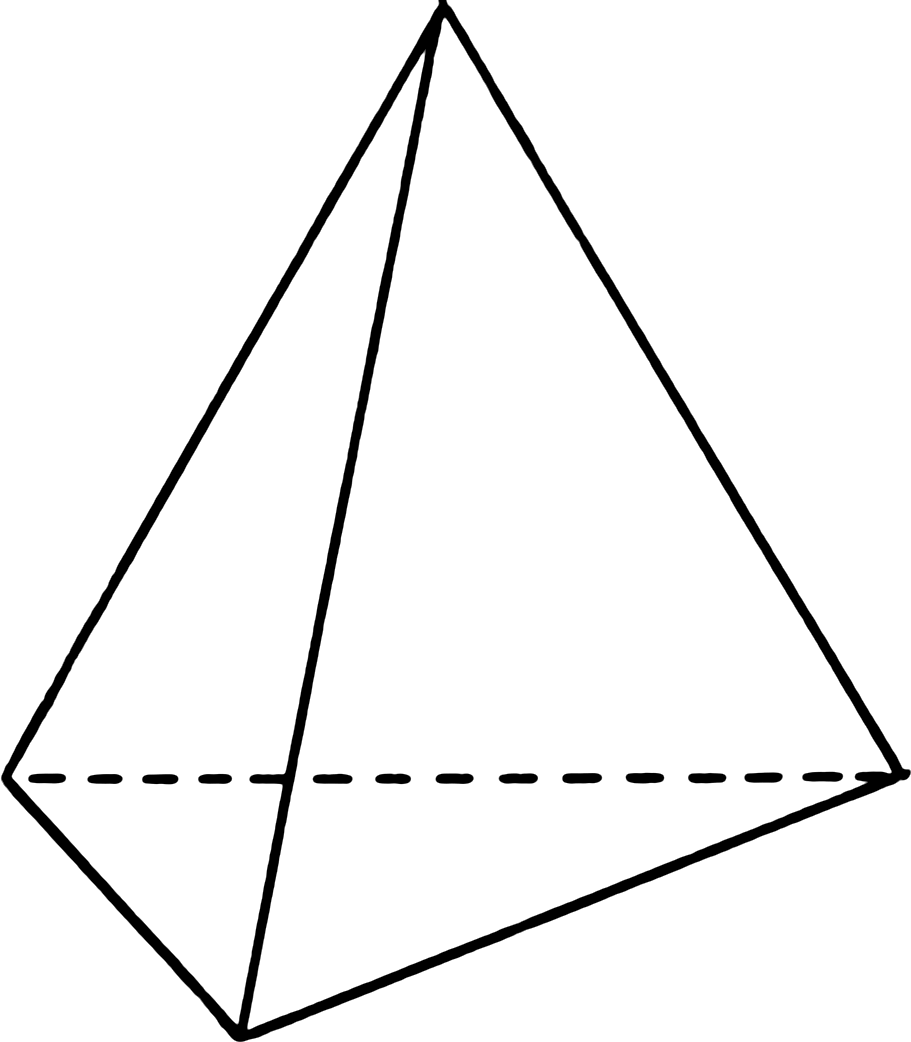
\includegraphics[width = 1.2in]{tetra}
\end{center}
\end{problem}

\textbf{Solution:}
We know the area of an equilateral triangle with side $s$ is just

$$\frac{s^2\sqrt{3}}{4}.$$

Now we just need to find the height from the base of the tetrahedron to the top vertex. This easy to do once we view the tetrahedron from the top vertex, because we find out that the top vertex height drops directly down to the center of the equilateral triangle. We can then use one of the edges and the distance from the center of the equilateral triangle to one of its sides along with the height to build a right triangle. The height is then just 
$$\sqrt{s^2-\left(\frac{s}{\sqrt{3}}\right)^2}=s\sqrt{\frac{2}{3}}$$
and the volume is 
$$\frac{1}{3}\cdot s\sqrt{\frac{2}{3}}\cdot \frac{s^2\sqrt{3}}{4} = \boxed{\frac{s^3\sqrt{2}}{12}}$$
DON'T ever forget the $\frac{1}{3}$ factor for the volume of pyramids.

As you can see, 3D geometry problems are really just a bunch of 2D problems, so whenever you have a 3D object, try to dissect it down as much as possible! Try looking at the object in different perspectives, chopping it up, and drawing in extra lines. Also, sometimes the 3D geometry problem is just a setup for an algebra problem. Unfortunately, this algebra can sometimes get \textit{very ugly}. But what can you do? Math all relies on each other, and pure geometry can't always get you to the final answer.


\subsection{Euler's Formula} %https://www.artofproblemsolving.com/wiki/index.php?title=Euler%27s_Polyhedral_Formula
Euler's Formula states that 
\begin{equation}
    F+V-E=2,
\end{equation}
where $F$ is the number of faces, $V$ is the number of vertices, and $E$ is the number of edges.

\begin{problem}
Fill in the following table to verify Euler's Formula

\begin{figure}[H]
    
  \begin{minipage}[]{0.24\textwidth}
    \centering
    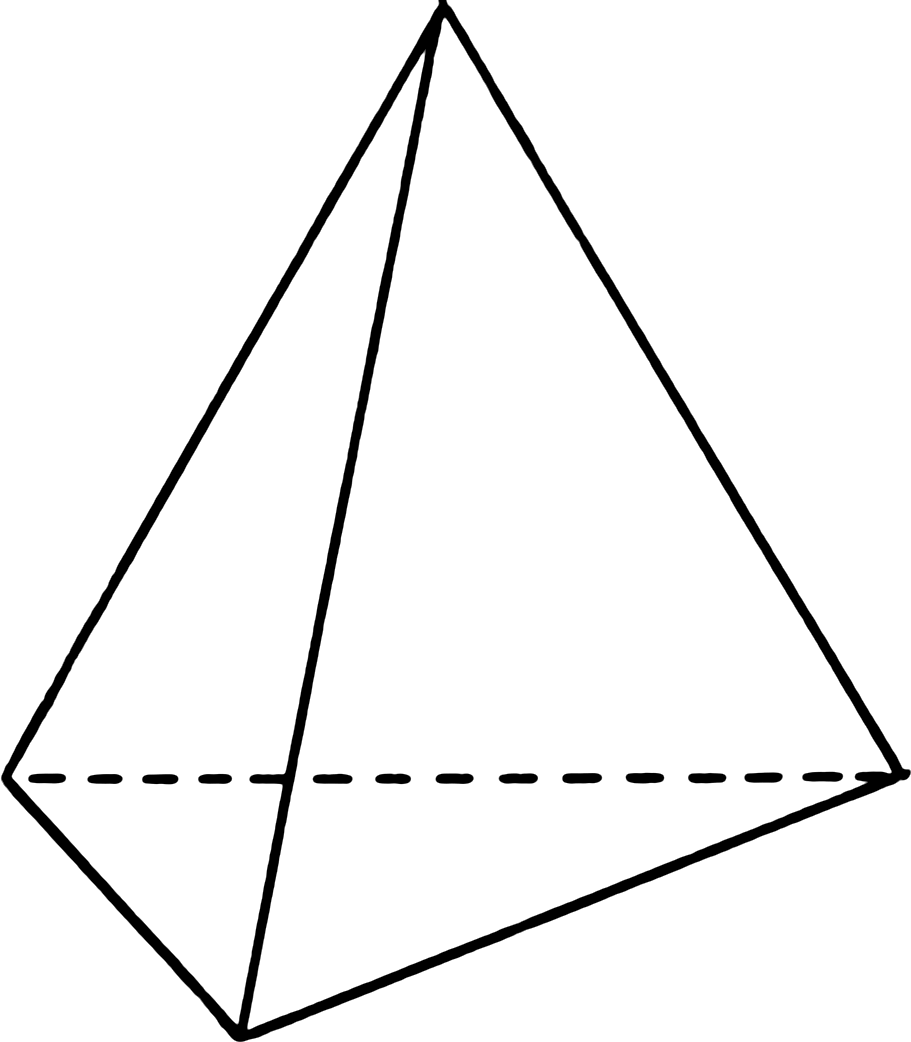
\includegraphics[width = 1.2in]{tetra}
    \caption{Tetrahedron}
    \label{fig:tetra}
  \end{minipage}
  \begin{minipage}[]{0.22\textwidth}
    \centering
    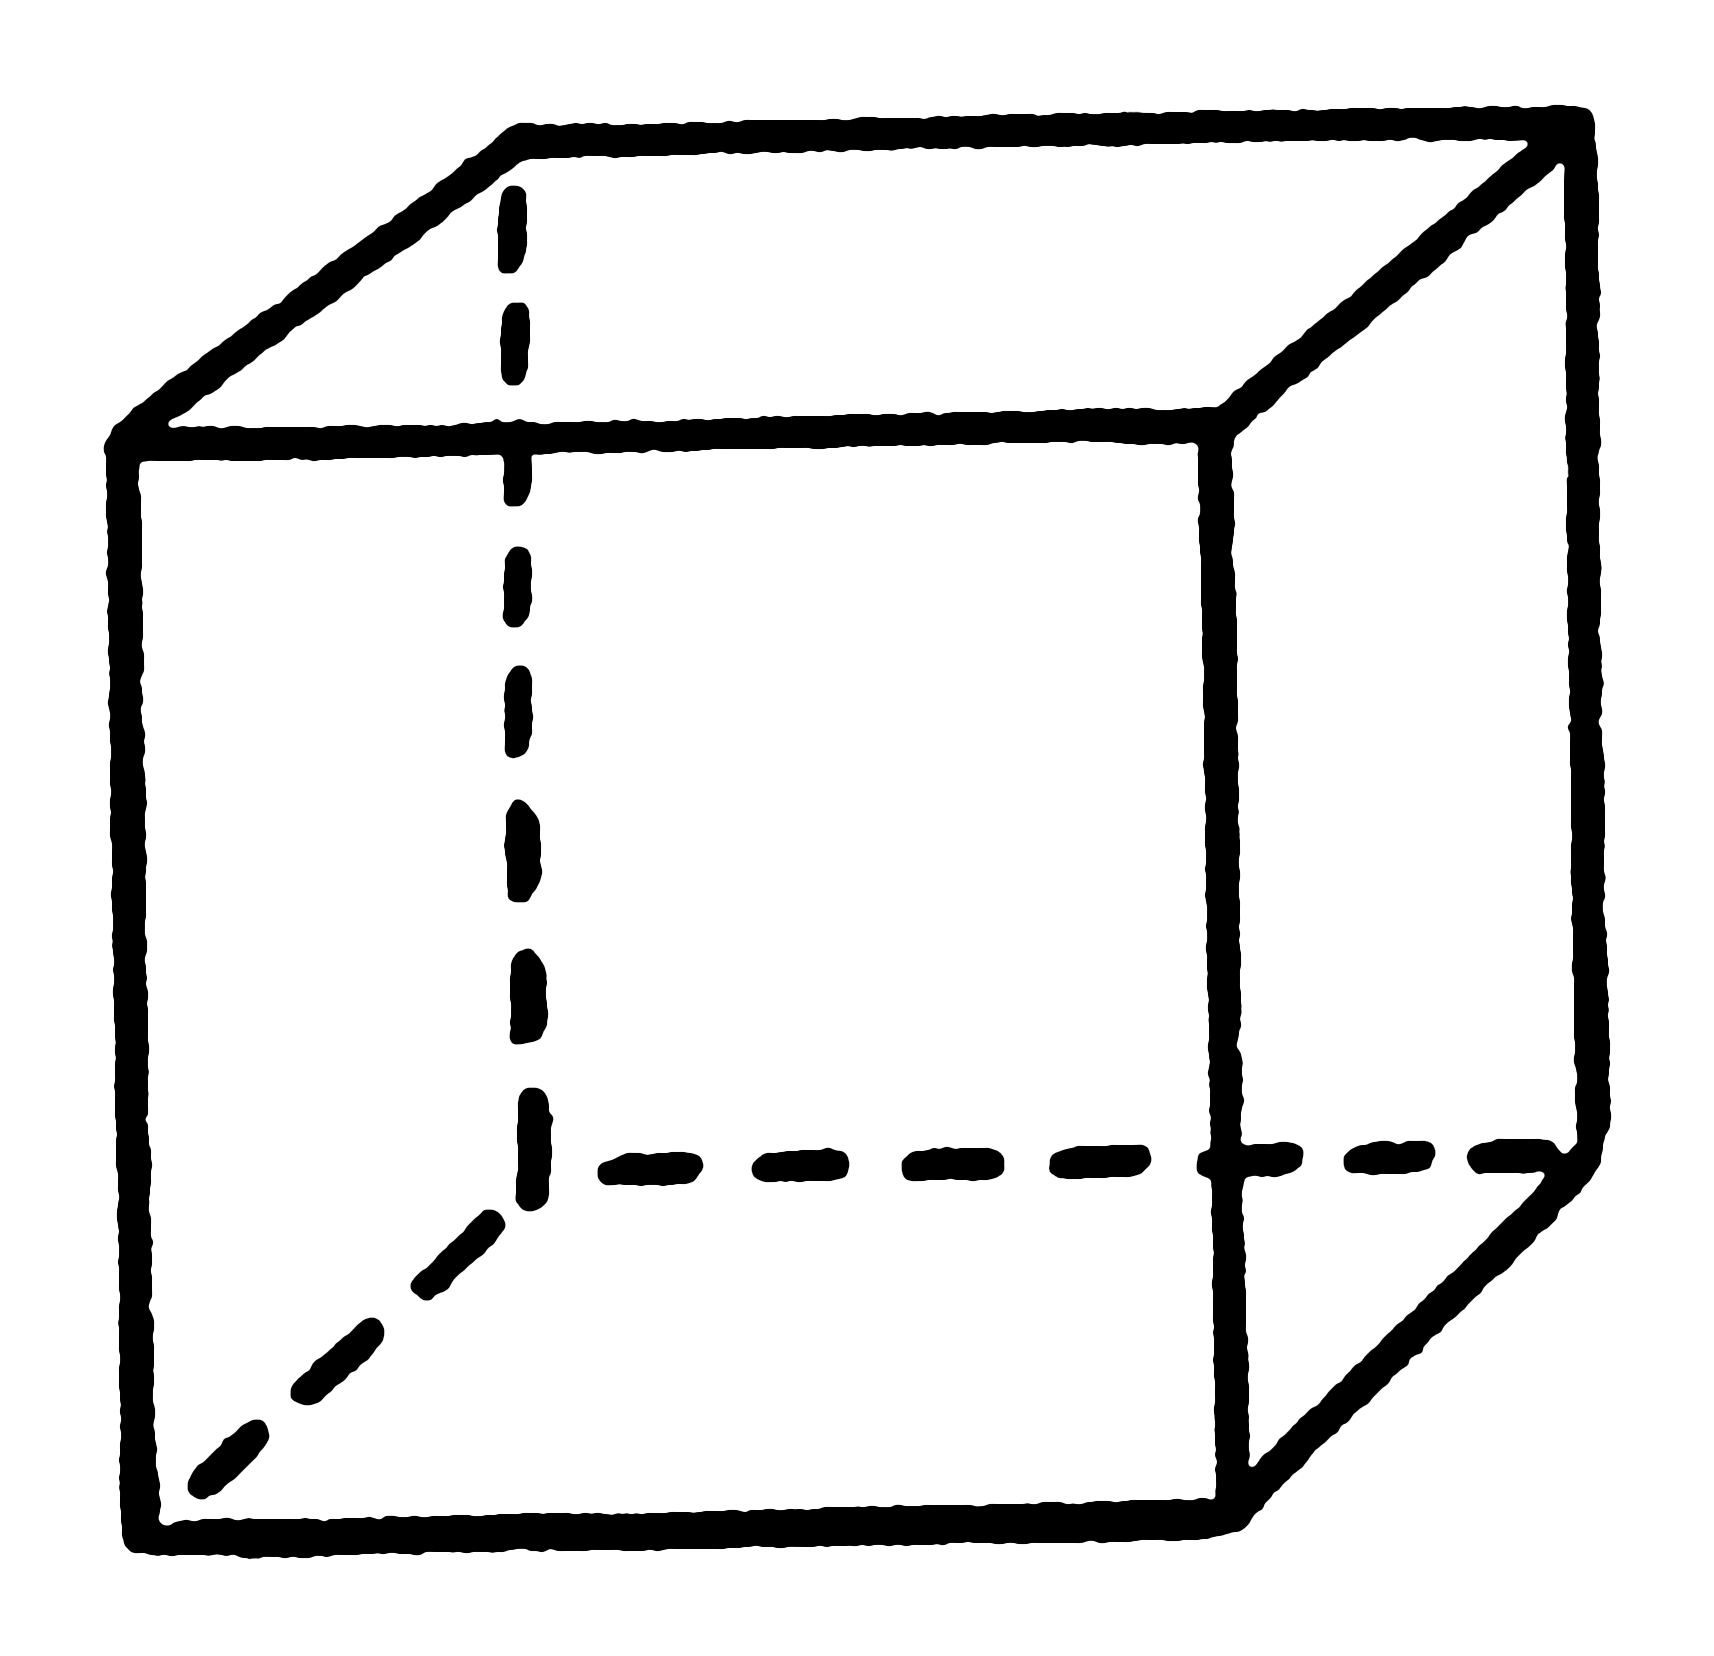
\includegraphics[width=1.4in]{cube2}
    \caption{Cube}
    \label{fig:cube}
  \end{minipage}
  \begin{minipage}[]{0.25\textwidth}
    \centering
    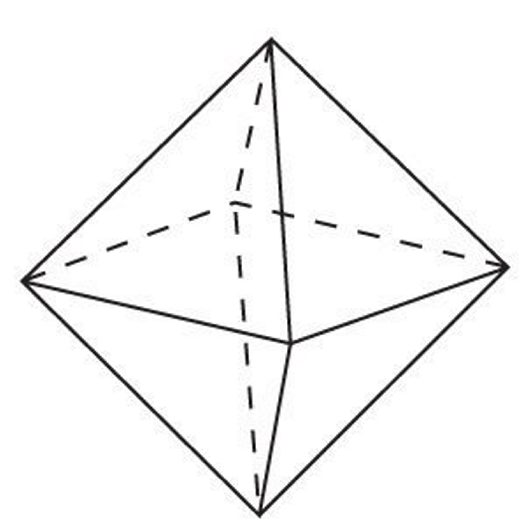
\includegraphics[width = 1.37in]{octa}
    \caption{Octahedron}
    \label{fig:octa}
  \end{minipage}
  \begin{minipage}[]{0.25\textwidth}
    \centering
    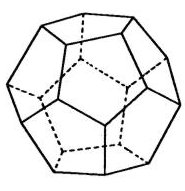
\includegraphics[width=1.35in]{dodec2}
    \caption{Dodecahedron}
    \label{fig:dodec}
  \end{minipage}
  
\end{figure}

\centering
\def\arraystretch{1.5}
$\begin{tabular}{|c|c|c|c|}\hline Shape & Vertices & Edges & Faces\\ 
\hline Tetrahedron &  & &  \\ 
\hline Cube &  &  & \\ 
\hline Octahedron &  &  & \\ 
\hline Dodecahedron & &  & \\ 
\hline 
\end{tabular}$
\end{problem}

\subsection{Problems}
%https://artofproblemsolving.com/wiki/index.php?title=Category:3D_Geometry_Problems

\begin{problem}
Find the equation of the line that passes through $(4, 5)$ and $(-11, 18)$ and find its slope and $y$-intercept.
\end{problem}

\begin{problem}
Find the distance between:
\begin{itemize}
    \item $(1,-10)$ and $(9,5)$
    \item $(3,-10)$ and $(19,-4)$
    \item $(2,-4,11)$ and $(7,6,-3)$
    \item $(1, 3, 2, -6, 7, 8)$ and $(-4, 4, 2, 4, 7, 11)$
\end{itemize}
\end{problem}

\begin{problem}
Find the surface area and volume of an octahedron with side $s$.
\begin{center}
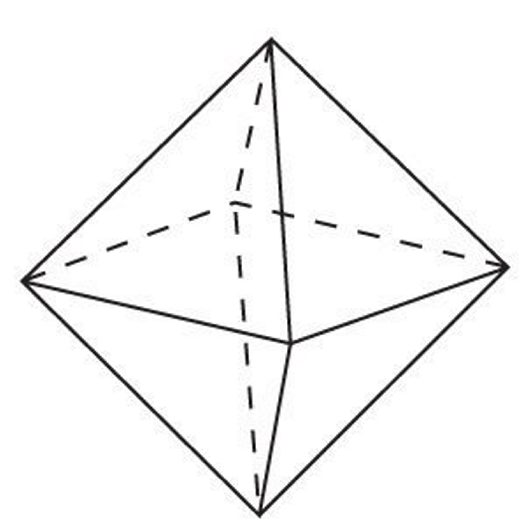
\includegraphics[width = 1.37in]{octa}
\end{center}
\end{problem}

\begin{problem}
The edges of a cube sum up to 144. What is the length of its spacial diagonal? \textit{Source: MATHCOUNTS}
\end{problem}

\begin{problem}
The surface area of a cube is twice its volume. Find the interior diagonal of the cube. \textit{Source: MATHCOUNTS}
\end{problem}

\begin{problem}
A cube is inscribed in a sphere, find the ratio of the volume of the cube to the sphere.
\end{problem}

\begin{problem}
A $5\times 8$ rectangle can be rolled up into a cylinder in two different ways. Find the ratio of the more voluminous cylinder to the smaller one. \textit{Source: MATHCOUNTS}
\end{problem}

\begin{problem}
A rope is wrapped exactly five times around a cylinder of radius 3 and height 20. What is the length of the rope?
\end{problem}

\begin{problem}
A right prism with height $h$ has bases that are regular hexagons with sides of length $12$. A vertex $A$ of the prism and its three adjacent vertices are the vertices of a triangular pyramid. The dihedral angle (the angle between the two planes) formed by the face of the pyramid that lies in a base of the prism and the face of the pyramid that does not contain $A$ measures $60$ degrees. Find $h^2$. \textit{Source: AIME}
\end{problem}

\begin{problem}
Buildoo is designing a new shape of brick. He constructs it by setting a brick cone with slant height 5 and base radius 4 on the ground, then cutting off a smaller cone with a cut parallel to the base of the cone (this forms a frustum). If the volume of Buildoo’s brick is $\frac{63\pi}{4}$, what is its surface area? \textit{Source: TJTST}
\end{problem}

\begin{problem}
A rectangular box has integer edge lengths. The sum of the numerical values of its volume, its surface area, and its twelve edge lenghths is 2015. Compute the length of the box's interior diagonal. \textit{Source: ARML}
\end{problem}

\begin{problem}
Corners are sliced off a unit cube so that the six faces each become regular octagons. What is the total volume of the removed tetrahedra?
\vspace{0.1in}
\begin{figure}[H]
    \centering
    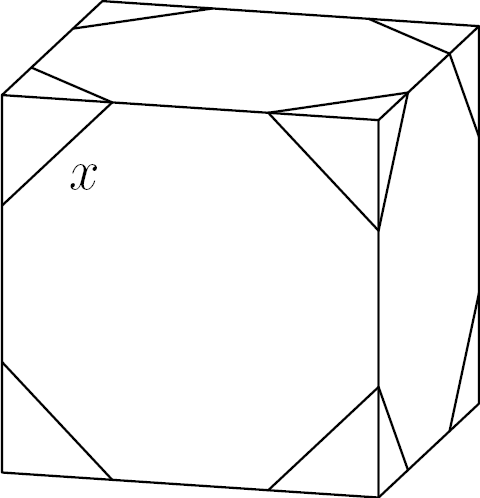
\includegraphics[width=1.7in]{cubetetra}
    \caption{Diagram for Problem \ref{pr:cubetetra}}
\end{figure}
\label{pr:cubetetra}
\end{problem}

\begin{problem}
Three mutually tangent spheres of radius $1$ rest on a horizontal plane. A sphere of radius $2$ rests on them. What is the distance from the plane to the top of the larger sphere? \textit{Source: AMC}
\end{problem}

\begin{problem}
Six spheres of radius $1$ are positioned so that their centers are at the vertices of a regular hexagon of side length $2$. The six spheres are internally tangent to a larger sphere whose center is the center of the hexagon. An eighth sphere is externally tangent to the six smaller spheres and internally tangent to the larger sphere. What is the radius of this eighth sphere? \textit{Source: AMC}
\end{problem}

\begin{problem}
Let $ABCD$ be a unit square. Let $E$ be the midpoint of $\overline{AB}$ and let $F$ be the midpoint of $\overline{BC}$. Find the area of the triangle bounded by the lines $\overline{EC}, \overline{AF}$, and $\overline{DF}$
\end{problem}